\documentclass[a4paper,12pt]{article}

\usepackage[utf8x]{inputenc}
\usepackage[T2A]{fontenc}
\usepackage[english, russian]{babel}

% Опционно, требует  apt-get install scalable-cyrfonts.*
% и удаления одной строчки в cyrtimes.sty
% Сточку не удалять!
% \usepackage{cyrtimes}

% Картнки и tikz
\usepackage{graphicx}
\usepackage{tikz}
\usetikzlibrary{snakes,arrows,shapes}


% Некоторая русификация.
\usepackage{misccorr}
\usepackage{indentfirst}
\renewcommand{\labelitemi}{\normalfont\bfseries{--}}

% Увы, поля придётся уменьшить из-за листингов.
\topmargin -1cm
\oddsidemargin -0.5cm
\evensidemargin -0.5cm
\textwidth 17cm
\textheight 24cm

\sloppy

% Оглавление в PDF
\usepackage[
bookmarks=true,
colorlinks=true, linkcolor=black, anchorcolor=black, citecolor=black, menucolor=black,filecolor=black, urlcolor=black,
unicode=true
]{hyperref}

% Для исходного кода в тексте
\newcommand{\Code}[1]{\texttt{#1}}


\title{Отчёт по лабораторной работе \\ <<Система доменных имён>>}
\author{Binh D. Nguyen}

\begin{document}

\maketitle

\tableofcontents

\section{Настройка системы DNS}

\subsection{Топология сети}

Топология сети и использыемые IP-адреса показаны на рис.~\ref{fig:network}.

\begin{figure}
\centering
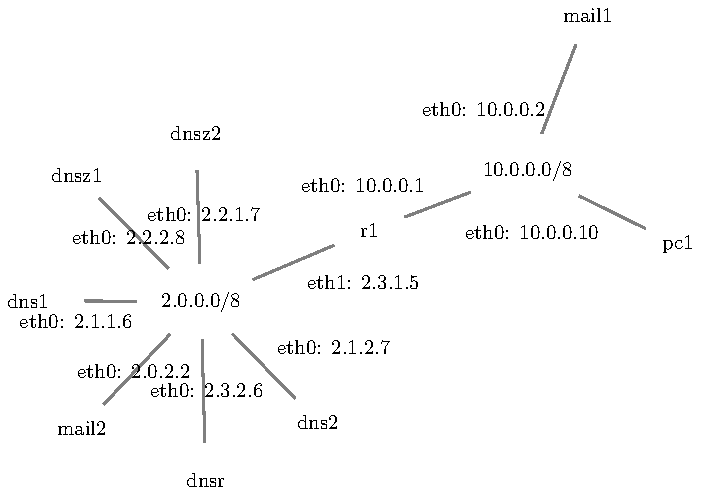
\includegraphics[width=\textwidth]{includes/network_gv.pdf}
\caption{Топология сети}
\label{fig:network}
\end{figure}

\subsection{Структура службы доменных имён}

Структура авторитетных серверов доменных имён показана на рис.~\ref{fig:dns}.

\begin{figure}
\centering
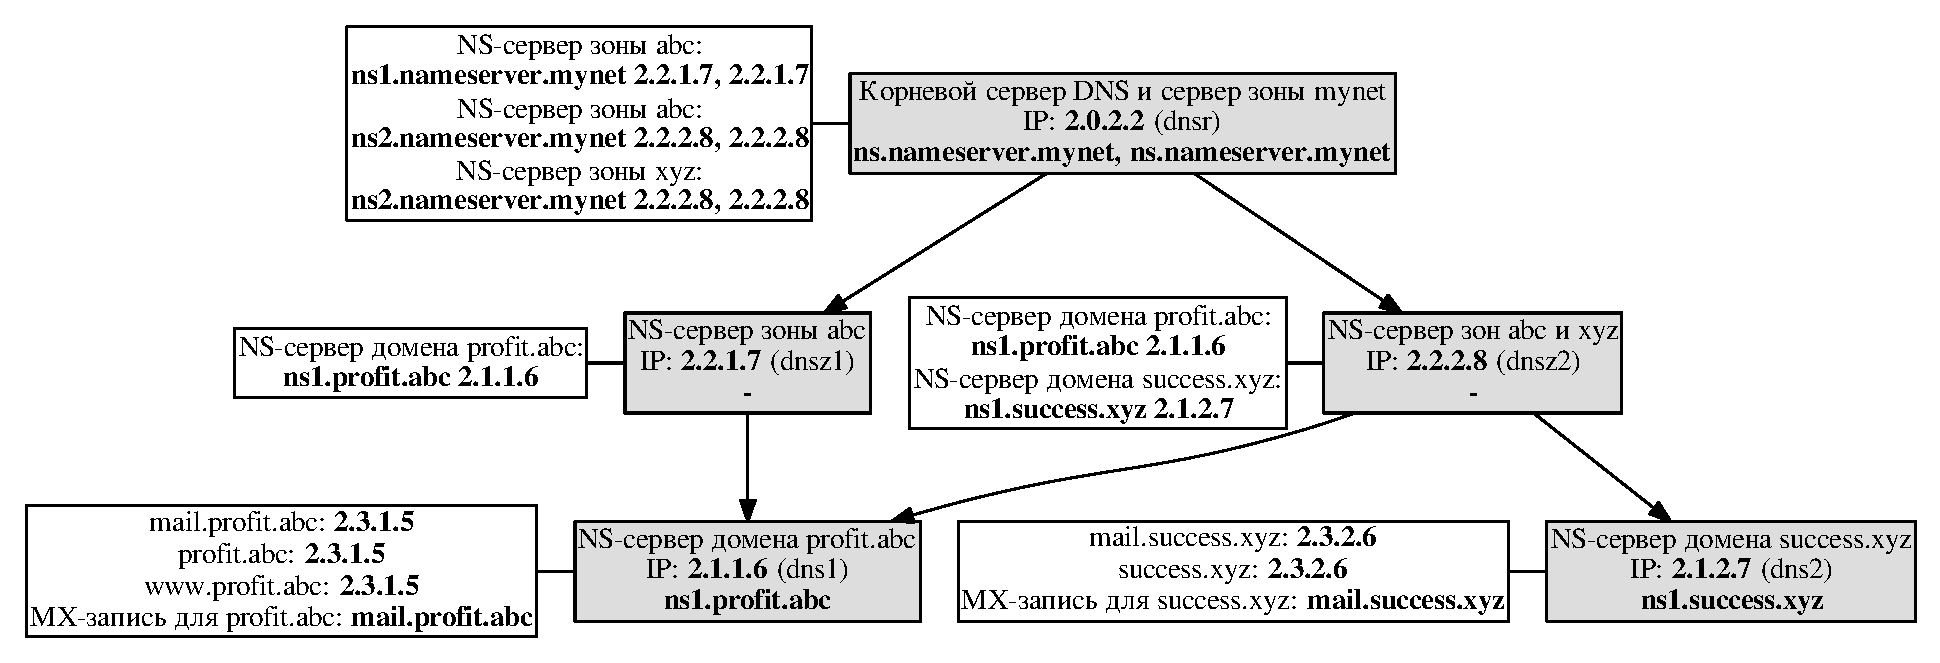
\includegraphics[width=\textwidth]{includes/dns_gv.pdf}
\caption{Структура службы доменных имён}
\label{fig:dns}
\end{figure}

\subsection{Прочие настройки}

Кеширующие DNS-серверы
\begin{itemize}
\item r1 (2.3.1.5, 10.0.0.1);
\item mail2 (2.3.2.6);
\end{itemize}

Развёрнутые SMTP-серверы и используемые ими кеширующие DNS-серверы.
\begin{itemize}
\item mail1 (2.3.1.5, 10.0.0.2) использует сервер на 10.0.0.1 (r1);
\item mail2 (2.3.2.6) использует сервер на 2.3.2.6 (самого себя);
\end{itemize}


\section{Проверка настройки службы доменных имён}

\subsection{Проверка настройки записи типа 'А' для домена 'success.xyz'}

(по цепочке опрашиваем с корневого сервера ручками)

Запросы шлем с r1

\begin{verbatim}
~# dig @2.0.2.2 success.xyz

; <<>> DiG 9.5.0-P2 <<>> @2.0.2.2 success.xyz
; (1 server found)
;; global options:  printcmd
;; Got answer:
;; ->>HEADER<<- opcode: QUERY, status: NOERROR, id: 65096
;; flags: qr rd; QUERY: 1, ANSWER: 0, AUTHORITY: 1, ADDITIONAL: 1
;; WARNING: recursion requested but not available

;; QUESTION SECTION:
;success.xyz.			IN	A

;; AUTHORITY SECTION:
xyz.			86400	IN	NS	ns2.nameserver.mynet.

;; ADDITIONAL SECTION:
ns2.nameserver.mynet.	86400	IN	A	2.2.2.8

;; Query time: 13 msec
;; SERVER: 2.0.2.2#53(2.0.2.2)
;; WHEN: Thu Dec  5 05:24:26 2019
;; MSG SIZE  rcvd: 79
\end{verbatim}

\begin{verbatim}
~# dig @2.2.2.8 success.xyz

; <<>> DiG 9.5.0-P2 <<>> @2.2.2.8 success.xyz
; (1 server found)
;; global options:  printcmd
;; Got answer:
;; ->>HEADER<<- opcode: QUERY, status: NOERROR, id: 30111
;; flags: qr rd; QUERY: 1, ANSWER: 0, AUTHORITY: 1, ADDITIONAL: 1
;; WARNING: recursion requested but not available

;; QUESTION SECTION:
;success.xyz.			IN	A

;; AUTHORITY SECTION:
success.xyz.		86400	IN	NS	ns1.success.xyz.

;; ADDITIONAL SECTION:
ns1.success.xyz.	86400	IN	A	2.1.2.7

;; Query time: 12 msec
;; SERVER: 2.2.2.8#53(2.2.2.8)
;; WHEN: Thu Dec  5 05:25:48 2019
;; MSG SIZE  rcvd: 63
\end{verbatim}

\begin{verbatim}
~# dig @2.1.2.7 success.xyz

; <<>> DiG 9.5.0-P2 <<>> @2.1.2.7 success.xyz
; (1 server found)
;; global options:  printcmd
;; Got answer:
;; ->>HEADER<<- opcode: QUERY, status: NOERROR, id: 25563
;; flags: qr aa rd; QUERY: 1, ANSWER: 1, AUTHORITY: 1, ADDITIONAL: 1
;; WARNING: recursion requested but not available

;; QUESTION SECTION:
;success.xyz.			IN	A

;; ANSWER SECTION:
success.xyz.		86400	IN	A	2.3.2.6

;; AUTHORITY SECTION:
success.xyz.		86400	IN	NS	ns1.success.xyz.

;; ADDITIONAL SECTION:
ns1.success.xyz.	86400	IN	A	2.1.2.7

;; Query time: 17 msec
;; SERVER: 2.1.2.7#53(2.1.2.7)
;; WHEN: Thu Dec  5 05:26:58 2019
;; MSG SIZE  rcvd: 79
\end{verbatim}

Итоговая проверка: опрашиваем кеширующий DNS-сервер.
Запрос шлем с pc1

\begin{verbatim}
~# dig @10.0.0.1 success.xyz

; <<>> DiG 9.5.0-P2 <<>> @10.0.0.1 success.xyz
; (1 server found)
;; global options:  printcmd
;; Got answer:
;; ->>HEADER<<- opcode: QUERY, status: NOERROR, id: 56697
;; flags: qr rd ra; QUERY: 1, ANSWER: 1, AUTHORITY: 0, ADDITIONAL: 0

;; QUESTION SECTION:
;success.xyz.			IN	A

;; ANSWER SECTION:
success.xyz.		86400	IN	A	2.3.2.6

;; Query time: 5 msec
;; SERVER: 10.0.0.1#53(10.0.0.1)
;; WHEN: Thu Dec  5 05:28:21 2019
;; MSG SIZE  rcvd: 45
\end{verbatim}

\begin{verbatim}
~# ping success.xyz -c 1
PING success.xyz (2.3.2.6) 56(84) bytes of data.
64 bytes from 2.3.2.6: icmp_seq=1 ttl=63 time=0.100 ms

--- success.xyz ping statistics ---
1 packets transmitted, 1 received, 0% packet loss, time 0ms
rtt min/avg/max/mdev = 0.100/0.100/0.100/0.000 ms

\end{verbatim}

\subsection{Проверка настройки записи типа 'A' для домена 'profit.abc'}

(по цепочке опрашиваем с корневого сервера ручками)
Запросы шлем с r1

\begin{verbatim}
~# dig @2.0.2.2 profit.abc

; <<>> DiG 9.5.0-P2 <<>> @2.0.2.2 profit.abc
; (1 server found)
;; global options:  printcmd
;; Got answer:
;; ->>HEADER<<- opcode: QUERY, status: NOERROR, id: 19819
;; flags: qr rd; QUERY: 1, ANSWER: 0, AUTHORITY: 2, ADDITIONAL: 2
;; WARNING: recursion requested but not available

;; QUESTION SECTION:
;profit.abc.			IN	A

;; AUTHORITY SECTION:
abc.			86400	IN	NS	ns1.nameserver.mynet.
abc.			86400	IN	NS	ns2.nameserver.mynet.

;; ADDITIONAL SECTION:
ns1.nameserver.mynet.	86400	IN	A	2.2.1.7
ns2.nameserver.mynet.	86400	IN	A	2.2.2.8

;; Query time: 4 msec
;; SERVER: 2.0.2.2#53(2.0.2.2)
;; WHEN: Thu Dec  5 05:33:54 2019
;; MSG SIZE  rcvd: 112
\end{verbatim}

\begin{verbatim}
~# dig @2.2.1.7 profit.abc

; <<>> DiG 9.5.0-P2 <<>> @2.2.1.7 profit.abc
; (1 server found)
;; global options:  printcmd
;; Got answer:
;; ->>HEADER<<- opcode: QUERY, status: NOERROR, id: 26783
;; flags: qr rd; QUERY: 1, ANSWER: 0, AUTHORITY: 1, ADDITIONAL: 1
;; WARNING: recursion requested but not available

;; QUESTION SECTION:
;profit.abc.			IN	A

;; AUTHORITY SECTION:
profit.abc.		86400	IN	NS	ns1.profit.abc.

;; ADDITIONAL SECTION:
ns1.profit.abc.		86400	IN	A	2.1.1.6

;; Query time: 7 msec
;; SERVER: 2.2.1.7#53(2.2.1.7)
;; WHEN: Thu Dec  5 05:35:00 2019
;; MSG SIZE  rcvd: 62
\end{verbatim}

\begin{verbatim}
~# dig @2.1.1.6 profit.abc

; <<>> DiG 9.5.0-P2 <<>> @2.1.1.6 profit.abc
; (1 server found)
;; global options:  printcmd
;; Got answer:
;; ->>HEADER<<- opcode: QUERY, status: NOERROR, id: 32097
;; flags: qr aa rd; QUERY: 1, ANSWER: 1, AUTHORITY: 1, ADDITIONAL: 1
;; WARNING: recursion requested but not available

;; QUESTION SECTION:
;profit.abc.			IN	A

;; ANSWER SECTION:
profit.abc.		86400	IN	A	2.3.1.5

;; AUTHORITY SECTION:
profit.abc.		86400	IN	NS	ns1.profit.abc.

;; ADDITIONAL SECTION:
ns1.profit.abc.		86400	IN	A	2.1.1.6

;; Query time: 5 msec
;; SERVER: 2.1.1.6#53(2.1.1.6)
;; WHEN: Thu Dec  5 05:35:10 2019
;; MSG SIZE  rcvd: 78
\end{verbatim}

Итоговая проверка: опрашиваем кеширующий DNS-сервер.
Запрос шлем с pc1

\begin{verbatim}
~# dig @10.0.0.1 profit.abc

; <<>> DiG 9.5.0-P2 <<>> @10.0.0.1 profit.abc
; (1 server found)
;; global options:  printcmd
;; Got answer:
;; ->>HEADER<<- opcode: QUERY, status: NOERROR, id: 52168
;; flags: qr rd ra; QUERY: 1, ANSWER: 1, AUTHORITY: 0, ADDITIONAL: 0

;; QUESTION SECTION:
;profit.abc.			IN	A

;; ANSWER SECTION:
profit.abc.		86400	IN	A	2.3.1.5

;; Query time: 23 msec
;; SERVER: 10.0.0.1#53(10.0.0.1)
;; WHEN: Thu Dec  5 05:37:12 2019
;; MSG SIZE  rcvd: 44
\end{verbatim}

\begin{verbatim}
~# ping profit.abc -c 1
PING profit.abc (2.3.1.5) 56(84) bytes of data.
64 bytes from 2.3.1.5: icmp_seq=1 ttl=64 time=0.056 ms

--- profit.abc ping statistics ---
1 packets transmitted, 1 received, 0% packet loss, time 0ms
rtt min/avg/max/mdev = 0.056/0.056/0.056/0.000 ms
\end{verbatim}

\section{Проверка работы почтовой системы}

\subsection{Проверка MX-записи для домена profit.abc}

Создали пользователей binh на узле mail1 и anna на узле mail2.
С узла pc1 отправили письмо на локальный SMTP-сервер (mail1) для адресата с адресом binh@profit.abc от адресата anna@success.xyz

\begin{verbatim}
2019-12-13 12:32:29 1ifk7J-0000I9-CB <= anna@success.xyz H=(localhost) [10.0.0.1] P=smtp S=303
2019-12-13 12:32:29 1ifk7J-0000I9-CB => binh <binh@profit.abc> R=local_user T=mail_spool
2019-12-13 12:32:29 1ifk7J-0000I9-CB Completed
\end{verbatim}

На машине с доменным именем mail1 появилось доставленное письмо.
\begin{verbatim}
From anna@success.xyz Fri Dec 13 12:32:29 2019
Return-path: <anna@success.xyz>
Envelope-to: binh@profit.abc
Delivery-date: Fri, 13 Dec 2019 12:32:29 +0000
Received: from [10.0.0.1] (helo=localhost)
	by mail1 with smtp (Exim 4.69)
	(envelope-from <anna@success.xyz>)
	id 1ifk7J-0000I9-CB
	for binh@profit.abc; Fri, 13 Dec 2019 12:32:29 +0000
Message-Id: <E1ifk7J-0000I9-CB@mail1>
From: anna@success.xyz
Date: Fri, 13 Dec 2019 12:32:29 +0000

Hello, sbn!
\end{verbatim}

Таким образом, доменная запись типа MX для домена profit.abc настроена верно.

\subsection{Проверка MX-записи для домена success.xyz}

Создали пользователей binh на узле mail1 и anna на узле mail2.
С узла pc1 отправили письмо на SMTP-сервер (mail2) для адресата с адресом anna@success.xyz

\begin{verbatim}
2019-12-28 16:06:35 1ifkeK-0000IJ-US <= binh@profit.abc H=[2.3.1.5] P=smtp S=184
2019-12-28 16:06:35 1ifkeK-0000IJ-US => anna <anna@success.xyz> R=local_user T=mail_spool
2019-12-28 16:06:35 1ifkeK-0000IJ-US Completed
\end{verbatim}

На машине с доменным именем mail2 появилось доставленное письмо.
\begin{verbatim}
From root@profit.abc Sat Dec 28 13:41:39 2019
Return-path: <root@profit.abc>
Envelope-to: anna@success.xyz
Delivery-date: Sat, 28 Dec 2019 13:41:39 +0000
Received: from [2.3.1.5] (helo=mail1)
	by mail2 with esmtp (Exim 4.69)
	(envelope-from <root@profit.abc>)
	id 1ilCLb-0000IF-Fz
	for anna@success.xyz; Sat, 28 Dec 2019 13:41:39 +0000
Received: from root by mail1 with local (Exim 4.69)
	(envelope-from <root@profit.abc>)
	id 1ilCLa-0000IF-RQ
	for anna@success.xyz; Sat, 28 Dec 2019 13:41:38 +0000
To: anna@success.xyz
Subject: test
Message-Id: <E1ilCLa-0000IF-RQ@mail1>
From: root <root@profit.abc>
Date: Sat, 28 Dec 2019 13:41:38 +0000

hello from binh

\end{verbatim}

Таким образом, доменная запись типа MX для домена success.xyz настроена верно.

\end{document}
